% ==== Strict Aliasing (and TBAA) ====
\section{Strict Aliasing (and TBAA)}

\begin{frame}{Strict aliasing}
  \begin{itemize}
  \item \textbf{Aliasing:} more than one name (pointer / reference) refers to same address.\\[1ex]
  \item \textbf{Strict Aliasing:} only pointers of the \textbf{same type} can point to the same object.
  \end{itemize}

  \vfill
  \begin{block}{[basic.lval], par. 11}
    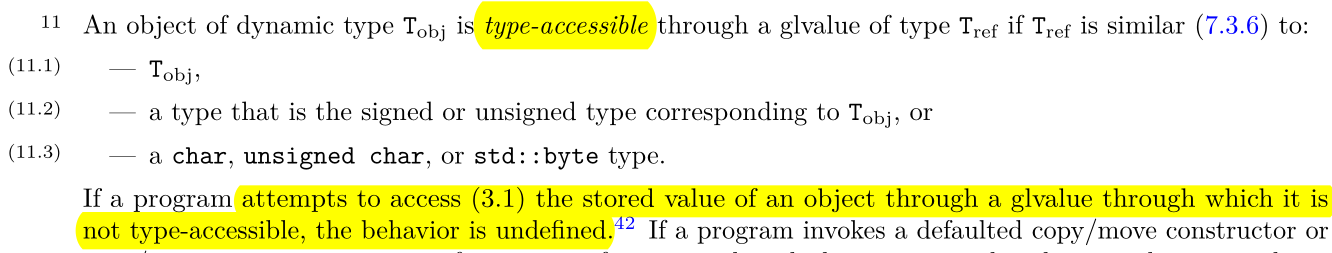
\includegraphics[width=\textwidth]{img/cplusplus_draft/basic.lval.11.png}
  \end{block}
\end{frame}

\begin{frame}[fragile]{A very obvious example}
  \lstinputlisting[style=c++]{code/violate_strict_aliasing.cpp}

  \begin{onlyenv}<2>
    \overlayLayer{
      \godbolt{https://godbolt.org/z/hj478h1aP}\\[1em]
      %
      \begin{columns}
        \column{.45\textwidth}\centering
        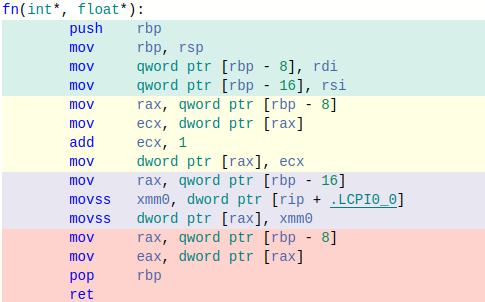
\includegraphics[width=\columnwidth]{img/violate_strict_aliasing_O0.png}\\
        (\texttt{-O0})
        %
        \column{.45\textwidth}\centering
        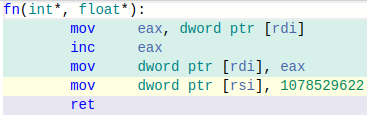
\includegraphics[width=\columnwidth]{img/violate_strict_aliasing_O2.png}\\
        (\texttt{-O2})
      \end{columns}
    }
  \end{onlyenv}
\end{frame}

\begin{frame}{A not-so-obvious example}
  BSD sockets: \inlineCode{sockaddr} vs. \inlineCode{sockaddr\_in}\\[2em]
  \textbf{Q: Strict aliasing violation (Y/N)?} ~\facepalm

  \vfill
  \lstinputlisting[linerange={5-10},style=c++]{code/BSDsockets_reinterpret_cast.cpp}
\end{frame}

\begin{frame}{Type-based Alias Analysis (TBAA)}
  \textbf{Alias analysis based on the type system of a high level language.}\\[1em]

  LLVM-specific, from \linkButton{https://github.com/llvm/llvm-project/blob/main/llvm/lib/Analysis/TypeBasedAliasAnalysis.cpp}{llvm/lib/Analysis/TypeBasedAliasAnalysis.cpp}:
  \begin{itemize}
  \item \textbf{Scalar TBAA:} alias analysis on fundamental datatype, \textbf{regardless of where it appears}.

  \item \textbf{Struct-path aware TBAA:} analysis takes into account \textbf{base type} (struct), \textbf{access type} (leaf, fundamental type), and its \textbf{offset}.
  \end{itemize}

  \vfill
  If you are interested, read the very clear 100+ code comment in there!
\end{frame}
